\section{Additional Background Material}\label{app:background}

The axioms, previously called the set $E$ of equations, of the SMTs
$\textbf{GLA}$, $\textbf{GAA}$ and $\textbf{GPA}$ introduced in
Section~\ref{sec:bg} are:

\begingroup
\tikzset{
		axpic/.style={baseline=(current bounding box.center), x=0.6cm, y=0.52cm, line cap=round},
		boxnode/.style={rounded rectangle, fill=white, draw=black, inner sep=2pt, anchor=center}
	}

	\medskip
	\noindent\fbox{\begin{minipage}{0.97\linewidth}
			\begin{center}\textbf{$\mathbf{GLA}$ axioms}\quad{\footnotesize\cite{paixao2022highlevel,bonchi2017interacting}}\end{center}

			\textit{White commutative monoid (addition $\oplus$, unit $\circ$).}
			\begin{center}\begin{tabular}{r@{\quad}c@{\;$=$\;}c}
					(assoc) &
                    \begin{tikzpicture}
                      \begin{scope}[shift={(0.000,1.000)}]
                      \pic (g1) at (0.500,0.500) {multiplication};
                      \end{scope}
                      \coordinate (id_in_2) at (0,0.500);
                      \coordinate (id_out_3) at (1.000,0.500);
                      \draw (id_in_2) -- (id_out_3);
                      \begin{scope}[shift={(1.250,0.500)}]
                      \pic (g4) at (0.500,0.500) {multiplication};
                      \end{scope}
                      \draw (g1-out-0) to[out=0,in=180] (g4-in-0);
                      \draw (id_out_3) to[out=0,in=180] (g4-in-1);
                    \end{tikzpicture}
					        &
                    \begin{tikzpicture}
                      \begin{scope}[shift={(0.000,1.000)}]
                      \coordinate (id_in_1) at (0,0.500);
                      \coordinate (id_out_2) at (1.000,0.500);
                      \draw (id_in_1) -- (id_out_2);
                      \end{scope}
                      \pic (g3) at (0.500,0.500) {multiplication};
                      \begin{scope}[shift={(1.250,0.500)}]
                      \pic (g4) at (0.500,0.500) {multiplication};
                      \end{scope}
                      \draw (id_out_2) to[out=0,in=180] (g4-in-0);
                      \draw (g3-out-0) to[out=0,in=180] (g4-in-1);
                    \end{tikzpicture}
					\\[3mm]
					(comm)  &
                    \begin{tikzpicture}
                      \coordinate (sw_in_top_1) at (0,1.000);
                      \coordinate (sw_in_bottom_2) at (0,0.000);
                      \coordinate (sw_out_top_3) at (1.000,1.000);
                      \coordinate (sw_out_bottom_4) at (1.000,0.000);
                      \draw (sw_in_bottom_2) .. controls (0.500,0.000) and (0.500,1.000) .. (sw_out_top_3);
                      \draw (sw_in_top_1) .. controls (0.500,1.000) and (0.500,0.000) .. (sw_out_bottom_4);
                      \begin{scope}[shift={(1.250,0.000)}]
                      \pic (g5) at (0.500,0.500) {multiplication};
                      \end{scope}
                      \draw (sw_out_top_3) to[out=0,in=180] (g5-in-0);
                      \draw (sw_out_bottom_4) to[out=0,in=180] (g5-in-1);
                    \end{tikzpicture}
					        &
                    \begin{tikzpicture}
                      \pic (g1) at (0.500,0.500) {multiplication};
                    \end{tikzpicture}
					\\[3mm]
					(unit)  &
                    \begin{tikzpicture}
                      \begin{scope}[shift={(0.000,1.000)}]
                      \pic (g1) at (0.500,0.500) {zero};
                      \end{scope}
                      \coordinate (id_in_2) at (0,0.500);
                      \coordinate (id_out_3) at (1.000,0.500);
                      \draw (id_in_2) -- (id_out_3);
                      \begin{scope}[shift={(1.250,0.500)}]
                      \pic (g4) at (0.500,0.500) {multiplication};
                      \end{scope}
                      \draw (g1-out-0) to[out=0,in=180] (g4-in-0);
                      \draw (id_out_3) to[out=0,in=180] (g4-in-1);
                    \end{tikzpicture}
					        &
                    \begin{tikzpicture}
                      \coordinate (id_in_1) at (0,0.500);
                      \coordinate (id_out_2) at (1.000,0.500);
                      \draw (id_in_1) -- (id_out_2);
                    \end{tikzpicture}
				\end{tabular}\end{center}

			\textit{Black cocommutative comonoid (copy, counit $\bullet$).}
			\begin{center}\begin{tabular}{r@{\quad}c@{\;$=$\;}c}
					(coassoc) &
                    \begin{tikzpicture}
                      \pic (g1) at (0.500,0.500) {copy};
                      \begin{scope}[shift={(1.250,0.000)}]
                      \pic (g2) at (0.500,0.500) {copy};
                      \end{scope}
                      \coordinate (id_in_3) at (1.250,1.000);
                      \coordinate (id_out_4) at (2.250,1.000);
                      \draw (id_in_3) -- (id_out_4);
                      \draw (g1-out-0) to[out=0,in=180] (g2-in-0);
                      \draw (g1-out-1) to[out=0,in=180] (id_in_3);
                    \end{tikzpicture}
					          &
                    \begin{tikzpicture}
                      \begin{scope}[shift={(0.000,1.000)}]
                      \pic (g1) at (0.500,0.500) {copy};
                      \end{scope}
                      \begin{scope}[shift={(1.250,0.000)}]
                      \pic (g2) at (0.500,0.500) {copy};
                      \end{scope}
                      \coordinate (id_in_3) at (1.250,0.000);
                      \coordinate (id_out_4) at (2.250,0.000);
                      \draw (id_in_3) -- (id_out_4);
                      \draw (g1-out-1) to[out=0,in=180] (g2-in-0);
                      \draw (g1-out-0) to[out=0,in=180] (id_in_3);
                    \end{tikzpicture}
					\\[3mm]
					(cocomm)  &
                    \begin{tikzpicture}
                      \pic (g1) at (0.500,0.500) {copy};
                      \coordinate (sw_in_top_1) at (1.000,1.000);
                      \coordinate (sw_in_bottom_2) at (1.000,0.000);
                      \coordinate (sw_out_top_3) at (2.000,1.000);
                      \coordinate (sw_out_bottom_4) at (2.000,0.000);
                      \draw (g1-out-1) to[out=0,in=180] (sw_in_top_1);
                      \draw (g1-out-0) to[out=0,in=180] (sw_in_bottom_2);
                      \draw (sw_in_bottom_2) .. controls (1.500,0.000) and (1.500,1.000) .. (sw_out_top_3);
                      \draw (sw_in_top_1) .. controls (1.500,1.000) and (1.500,0.000) .. (sw_out_bottom_4);
                    \end{tikzpicture}
					          &
                    \begin{tikzpicture}
                      \pic (g1) at (0.500,0.500) {copy};
                    \end{tikzpicture}
					\\[3mm]
					(counit)  &
                    \begin{tikzpicture}
                      \pic (g1) at (0.500,0.500) {copy};
                      \begin{scope}[shift={(1.250,0.500)}]
                      \pic (g2) at (0.500,0.500) {discard};
                      \end{scope}
                      \coordinate (id_in_3) at (1.250,0.000);
                      \coordinate (id_out_4) at (2.250,0.000);
                      \draw (id_in_3) -- (id_out_4);
                      \draw (g1-out-1) to[out=0,in=180] (g2-in-0);
                      \draw (g1-out-0) to[out=0,in=180] (id_in_3);
                    \end{tikzpicture}
					          &
                    \begin{tikzpicture}
                      \coordinate (id_in_1) at (0,0.500);
                      \coordinate (id_out_2) at (1.000,0.500);
                      \draw (id_in_1) -- (id_out_2);
                    \end{tikzpicture}
				\end{tabular}\end{center}

			\textit{Bialgebra / Hopf (white over black).}
			\begin{center}\begin{tabular}{r@{\quad}c@{\;$=$\;}c}
					(B1)       &
                    \begin{tikzpicture}
                      \pic (g1) at (0.500,0.500) {multiplication};
                      \begin{scope}[shift={(1.250,0.000)}]
                      \pic (g2) at (0.500,0.500) {copy};
                      \end{scope}
                      \draw (g1-out-0) to[out=0,in=180] (g2-in-0);
                    \end{tikzpicture}
					           &
                    \begin{tikzpicture}
                      \begin{scope}[shift={(0.000,1.500)}]
                      \pic (g1) at (0.500,0.500) {copy};
                      \end{scope}
                      \begin{scope}[shift={(0.000,0.000)}]
                      \pic (g2) at (0.500,0.500) {copy};
                      \end{scope}
                      \begin{scope}[shift={(1.750,1.500)}]
                      \pic (g3) at (0.500,0.500) {multiplication};
                      \end{scope}
                      \begin{scope}[shift={(1.750,0.000)}]
                      \pic (g4) at (0.500,0.500) {multiplication};
                      \end{scope}
                      \draw (g1-out-1) to[out=0,in=180] (g3-in-0);
                      \draw (g2-out-0) to[out=0,in=180] (g4-in-1);
                      \draw (g1-out-0) to[out=0,in=180] (g4-in-0);
                      \draw (g2-out-1) to[out=0,in=180] (g3-in-1);
                    \end{tikzpicture}
					\\[3mm]
					(B2)       &
                    \begin{tikzpicture}
                      \pic (g1) at (0.500,0.500) {multiplication};
                      \begin{scope}[shift={(1.250,0.500)}]
                      \pic (g2) at (0.500,0.500) {discard};
                      \end{scope}
                      \draw (g1-out-0) to[out=0,in=180] (g2-in-0);
                    \end{tikzpicture}
					           &
                    \begin{tikzpicture}
                      \begin{scope}[shift={(0.000,0.700)}]
                      \pic (g1) at (0.500,0.500) {discard};
                      \end{scope}
                      \begin{scope}[shift={(0.000,-0.700)}]
                      \pic (g2) at (0.500,0.500) {discard};
                      \end{scope}
                    \end{tikzpicture}
					\\[3mm]
					(B3)       &
                    \begin{tikzpicture}
                      \pic (g1) at (0.500,0.500) {zero};
                      \begin{scope}[shift={(1.250,0.000)}]
                      \pic (g2) at (0.500,0.500) {copy};
                      \end{scope}
                      \draw (g1-out-0) to[out=0,in=180] (g2-in-0);
                    \end{tikzpicture}
					           &
                    \begin{tikzpicture}
                      \begin{scope}[shift={(0.000,0.700)}]
                      \pic (g1) at (0.500,0.500) {zero};
                      \end{scope}
                      \begin{scope}[shift={(0.000,-0.700)}]
                      \pic (g2) at (0.500,0.500) {zero};
                      \end{scope}
                    \end{tikzpicture}
					\\[3mm]
					(B4, unit) &
                    \begin{tikzpicture}
                      \pic (g1) at (0.500,0.500) {zero};
                      \begin{scope}[shift={(1.250,0.000)}]
                      \pic (g2) at (0.500,0.500) {discard};
                      \end{scope}
                      \draw (g1-out-0) to[out=0,in=180] (g2-in-0);
                    \end{tikzpicture}
					           &
                    \begin{tikzpicture}
                      \path (0,0) rectangle (1.000,1.000);
                    \end{tikzpicture}
				\end{tabular}\end{center}

			\textit{Frobenius and special law (copy structure; the addition structure is dual).}
			\begin{center}\begin{tabular}{r@{\quad}c@{\;$=$\;}c}
					(Frob)    &
                    \begin{tikzpicture}
                      \begin{scope}[shift={(0.000,1.000)}]
                      \pic (g1) at (0.500,0.500) {copy};
                      \end{scope}
                      \begin{scope}[shift={(1.250,0.000)}]
                      \pic (g2) at (0.500,0.500) {cocopy};
                      \end{scope}
                      \coordinate (id_in_3) at (1.000,1.500);
                      \coordinate (id_out_4) at (2.750,1.500);
                      \draw (id_in_3) -- (id_out_4);
                      \coordinate (id_in_5) at (1.000,0.000);
                      \coordinate (id_out_6) at (2.750,0.000);
                      \draw (id_in_5) -- (id_out_6);
                      \draw (g1-out-1) to[out=0,in=180] (g2-in-0);
                      \draw (g1-out-0) to[out=0,in=180] (id_in_3);
                      \draw (id_out_6) to[out=0,in=0] (g2-in-1);
                    \end{tikzpicture}
					          &
                    \begin{tikzpicture}
                      \pic (g1) at (0.500,0.500) {cocopy};
                      \begin{scope}[shift={(1.250,0.000)}]
                      \pic (g2) at (0.500,0.500) {copy};
                      \end{scope}
                      \draw (g1-out-0) to[out=0,in=180] (g2-in-0);
                    \end{tikzpicture}
					\\[3mm]
					(special) &
                    \begin{tikzpicture}
                      \pic (g1) at (0.500,0.500) {copy};
                      \begin{scope}[shift={(1.250,0.000)}]
                      \pic (g2) at (0.500,0.500) {cocopy};
                      \end{scope}
                      \draw (g1-out-0) to[out=0,in=180] (g2-in-0);
                      \draw (g1-out-1) to[out=0,in=180] (g2-in-1);
                    \end{tikzpicture}
					          &
                    \begin{tikzpicture}
                      \coordinate (id_in_1) at (0,0.500);
                      \coordinate (id_out_2) at (1.000,0.500);
                      \draw (id_in_1) -- (id_out_2);
                    \end{tikzpicture}
				\end{tabular}\end{center}

			\textit{Scalars and antipode ($\text{-}1$).}
			\begin{center}\begin{tabular}{r@{\quad}c@{\;$=$\;}c}
					(s.\,add)  &
                    \begin{tikzpicture}
                      \pic (g1) at (0.500,0.500) {copy};
                      \begin{scope}[shift={(1.250,0.700)}]
                      \pic [val=k] (g2) at (0.500,0.500) {scalar};
                      \end{scope}
                      \begin{scope}[shift={(1.250,-0.700)}]
                      \pic [val=l] (g3) at (0.500,0.500) {scalar};
                      \end{scope}
                      \begin{scope}[shift={(2.750,0.000)}]
                      \pic (g4) at (0.500,0.500) {multiplication};
                      \end{scope}
                      \draw (g1-out-1) to[out=0,in=180] (g2-in-0);
                      \draw (g1-out-0) to[out=0,in=180] (g3-in-0);
                      \draw (g2-out-0) to[out=0,in=180] (g4-in-0);
                      \draw (g3-out-0) to[out=0,in=180] (g4-in-1);
                    \end{tikzpicture}
					           &
                    \begin{tikzpicture}
                      \pic [val={k+l}] (g1) at (0.500,0.500) {scalar};
                    \end{tikzpicture}
					\\[3mm]
					(s.\,mult) &
                    \begin{tikzpicture}
                      \pic [val=k] (g1) at (0.500,0.500) {scalar};
                      \begin{scope}[shift={(1.250,0.000)}]
                      \pic [val=l] (g2) at (0.500,0.500) {scalar};
                      \end{scope}
                      \draw (g1-out-0) to[out=0,in=180] (g2-in-0);
                    \end{tikzpicture}
					           &
                    \begin{tikzpicture}
                      \pic [val={kl}] (g1) at (0.500,0.500) {scalar};
                    \end{tikzpicture}
					\\[3mm]
					(antipode) &
                    \begin{tikzpicture}
                      \pic (g1) at (0.500,0.500) {copy};
                      \begin{scope}[shift={(1.250,-0.700)}]
                      \pic [val={\text{-}1}] (g2) at (0.500,0.500) {scalar};
                      \end{scope}
                      \begin{scope}[shift={(2.750,0.000)}]
                      \pic (g3) at (0.500,0.500) {multiplication};
                      \end{scope}
                      \coordinate (id_in_4) at (1.250,1.200);
                      \coordinate (id_out_5) at (2.750,1.200);
                      \draw (id_in_4) -- (id_out_5);
                      \draw (g1-out-1) to[out=0,in=180] (id_in_4);
                      \draw (g1-out-0) to[out=0,in=180] (g2-in-0);
                      \draw (id_out_5) to[out=0,in=180] (g3-in-0);
                      \draw (g2-out-0) to[out=0,in=180] (g3-in-1);
                    \end{tikzpicture}
					           &
                    \begin{tikzpicture}
                      \pic (g1) at (0.500,0.500) {discard};
                      \begin{scope}[shift={(1.250,0.000)}]
                      \pic (g2) at (0.500,0.500) {zero};
                      \end{scope}
                    \end{tikzpicture}
				\end{tabular}\end{center}
		\end{minipage}}

	\medskip
	\noindent\fbox{\begin{minipage}{0.97\linewidth}
			\begin{center}\textbf{$\mathbf{GAA}$ axioms (in addition to $\mathbf{GLA}$)}\quad{\footnotesize\cite{bonchi2019affine}}\end{center}
			The affine generator $\rtop$ (a point $0\to 1$, drawn as the empty box) is a comonoid homomorphism:
			\begin{center}\begin{tabular}{r@{\quad}c@{\;$=$\;}c}
					(aff.\,copy) &
                    \begin{tikzpicture}
                      \pic (g1) at (0.500,0.500) {affine};
                      \begin{scope}[shift={(1.250,0.000)}]
                      \pic (g2) at (0.500,0.500) {copy};
                      \end{scope}
                      \draw (g1-out-0) to[out=0,in=180] (g2-in-0);
                    \end{tikzpicture}
					             &
                    \begin{tikzpicture}
                      \begin{scope}[shift={(0.000,0.700)}]
                      \pic (g1) at (0.500,0.500) {affine};
                      \end{scope}
                      \begin{scope}[shift={(0.000,-0.700)}]
                      \pic (g2) at (0.500,0.500) {affine};
                      \end{scope}
                    \end{tikzpicture}
					\\[3mm]
					(aff.\,del)  &
                    \begin{tikzpicture}
                      \pic (g1) at (0.500,0.500) {affine};
                      \begin{scope}[shift={(1.250,0.000)}]
                      \pic (g2) at (0.500,0.500) {discard};
                      \end{scope}
                      \draw (g1-out-0) to[out=0,in=180] (g2-in-0);
                    \end{tikzpicture}
					             &
                    \begin{tikzpicture}
                      \path (0,0) rectangle (1.000,1.000);
                    \end{tikzpicture}
				\end{tabular}\end{center}
		\end{minipage}}

	\medskip
	\noindent\fbox{
        \begin{minipage}{0.97\linewidth}
			\begin{center}\textbf{$\mathbf{GPA}$ axioms (in addition to $\mathbf{GAA}$)}\quad{\footnotesize\cite{bonchi2021polyhedral}}\end{center}
			The order primitive $\ge$ is a preorder compatible with the linear structure
			(transitivity; monoid and comonoid morphism; $0\ge 0$):
			\begin{center}\begin{tabular}{r@{\quad}c@{\;$=$\;}c}
					(trans)           &
                    \begin{tikzpicture}
                      \pic (g1) at (0.500,0.500) {ge};
                      \begin{scope}[shift={(1.250,0.000)}]
                      \pic (g2) at (0.500,0.500) {ge};
                      \end{scope}
                      \draw (g1-out-0) to[out=0,in=180] (g2-in-0);
                    \end{tikzpicture}
					                  &
                    \begin{tikzpicture}
                      \pic (g1) at (0.500,0.500) {ge};
                    \end{tikzpicture}
					\\[3mm]
					(mono.\,$\oplus$) &
                    \begin{tikzpicture}
                      \pic (g1) at (0.500,0.500) {multiplication};
                      \begin{scope}[shift={(1.250,0.000)}]
                      \pic (g2) at (0.500,0.500) {ge};
                      \end{scope}
                      \draw (g1-out-0) to[out=0,in=180] (g2-in-0);
                    \end{tikzpicture}
					                  &
                    \begin{tikzpicture}
                      \begin{scope}[shift={(0.000,0.800)}]
                      \pic (g1) at (0.500,0.500) {ge};
                      \end{scope}
                      \begin{scope}[shift={(0.000,-0.800)}]
                      \pic (g2) at (0.500,0.500) {ge};
                      \end{scope}
                      \begin{scope}[shift={(1.500,0.000)}]
                      \pic (g3) at (0.500,0.500) {multiplication};
                      \end{scope}
                      \draw (g1-out-0) to[out=0,in=180] (g3-in-0);
                      \draw (g2-out-0) to[out=0,in=180] (g3-in-1);
                    \end{tikzpicture}
					\\[3mm]
					(mono.\,copy)     &
                    \begin{tikzpicture}
                      \pic (g1) at (0.500,0.500) {copy};
                      \begin{scope}[shift={(1.250,0.800)}]
                      \pic (g2) at (0.500,0.500) {ge};
                      \end{scope}
                      \begin{scope}[shift={(1.250,-0.800)}]
                      \pic (g3) at (0.500,0.500) {ge};
                      \end{scope}
                      \draw (g1-out-1) to[out=0,in=180] (g2-in-0);
                      \draw (g1-out-0) to[out=0,in=180] (g3-in-0);
                    \end{tikzpicture}
					                  &
                    \begin{tikzpicture}
                      \pic (g1) at (0.500,0.500) {ge};
                      \begin{scope}[shift={(1.250,0.000)}]
                      \pic (g2) at (0.500,0.500) {copy};
                      \end{scope}
                      \draw (g1-out-0) to[out=0,in=180] (g2-in-0);
                    \end{tikzpicture}
					\\[3mm]
					(zero)            &
                    \begin{tikzpicture}
                      \pic (g1) at (0.500,0.500) {zero};
                      \begin{scope}[shift={(1.250,0.000)}]
                      \pic (g2) at (0.500,0.500) {ge};
                      \end{scope}
                      \draw (g1-out-0) to[out=0,in=180] (g2-in-0);
                    \end{tikzpicture}
					                  &
                    \begin{tikzpicture}
                      \pic (g1) at (0.500,0.500) {zero};
                    \end{tikzpicture}
				\end{tabular}\end{center}
			Together with reflexivity, antisymmetry and positivity of scalars; see \cite{bonchi2021polyhedral,bonchi2021.9farkas}.
		\end{minipage}
    }

\endgroup

Building on Definition~\ref{def:arrows}, we establish the following notation to ease the
burden of future proofs. We will denote an abstract diagram from $\overrightarrow{\textbf{GLA}}$ as

\begin{figure}[H]
    \centering
    \diagdef{
    \pic[val=A] {matrix};
}{
              \begin{scope}[shift={(0.000,1.000)}]
              \begin{scope}[shift={(0.000,1.000)}]
              \pic (g1) at (0.500,0.500) {copy};
              \end{scope}
              \pic (g2) at (0.500,0.500) {copy};
              \end{scope}
              \begin{scope}[shift={(1.250,0.000)}]
              \begin{scope}[shift={(0.000,1.000)}]
              \begin{scope}[shift={(0.000,1.000)}]
              \begin{scope}[shift={(0.000,1.000)}]
                  \pic (g3)[val=a_{1,1}] at (0.500,0.500) {scalar};
              \end{scope}
              \pic (g4)[val=a_{2,1}] at (0.500,0.500) {scalar};
              \end{scope}
              \pic (g5)[val=a_{1,2}] at (0.500,0.500) {scalar};
              \end{scope}
              \pic (g6)[val=a_{2,2}] at (0.500,0.500) {scalar};
              \end{scope}
              \draw (g1-out-0) to[out=0,in=180] (g3-in-0);
              \draw (g1-out-1) to[out=0,in=180] (g4-in-0);
              \draw (g2-out-0) to[out=0,in=180] (g5-in-0);
              \draw (g2-out-1) to[out=0,in=180] (g6-in-0);
              \begin{scope}[shift={(2.500,1.000)}]
              \begin{scope}[shift={(0.000,1.000)}]
              \pic (g7) at (0.500,0.500) {multiplication};
              \end{scope}
              \pic (g8) at (0.500,0.500) {multiplication};
              \end{scope}
              \draw (g3-out-0) to[out=0,in=180] (g7-in-0);
              \draw (g4-out-0) to[out=0,in=180] (g7-in-1);
              \draw (g5-out-0) to[out=0,in=180] (g8-in-0);
              \draw (g6-out-0) to[out=0,in=180] (g8-in-1);
}

\end{figure}

Which denotes any matrix A, or, more formally, denotes the relation $xAy \equiv Ax=y$. Analogously, we also depict any diagram from $\overrightarrow{\textbf{GAA}}$ as

\begin{figure}[H]
    \centering
    \diagdef{
    \pic[val=A] {relation};
}{
      \begin{scope}[shift={(0.625,1.000)}]
          \pic[val=A] (g1) at (0.500,0.500) {matrix};
      \end{scope}
      \pic (g2) at (0.500,0.500) {affine};
      \begin{scope}[shift={(1.250,0.000)}]
          \pic[val=b] (g3) at (0.500,0.500) {scalar};
      \end{scope}
      \draw (g2-out-0) to[out=0,in=180] (g3-in-0);
      \coordinate (a4) at (0.000,0 |- g1-in-0);
      \draw (g1-in-0) -- (a4);
      \coordinate (a5) at (2.250,0 |- g1-out-0);
      \draw (g1-out-0) -- (a5);
      \begin{scope}[shift={(2.500,0.500)}]
      \pic (g6) at (0.500,0.500) {multiplication};
      \end{scope}
      \draw (a5) to[out=0,in=180] (g6-in-0);
      \draw (g3-out-0) to[out=0,in=180] (g6-in-1);
}

\end{figure}

which denotes an affine transformation, also known as the relation $xAy \equiv Ax + b = y$.
The equivalent hold for their dual form in
$\overleftarrow{\textbf{GLA}}$ and $\overleftarrow{\textbf{GAA}}$.

\section{Omitted Proofs}\label{app:proofs}

\begin{proof}[Proof of Proposition~\ref{prop:relq}]
	Associativity follows from the distributivity of $\otimes$ over $\bigvee$:
	for $R:A\to B$, $S:B\to C$, $T:C\to D$,
	\[
		((T\circ S)\circ R)(a,d)
		= \bigvee_{b,c} R(a,b)\otimes S(b,c)\otimes T(c,d)
		= (T\circ (S\circ R))(a,d).
	\]
	The identity $1_A(a,b) = e$ if $a=b$ and $\bot$ otherwise satisfies $R\circ 1_A = R$
	since $e\otimes R(a,b) = R(a,b)$ and all remaining terms vanish.
	When $Q$ is commutative, the symmetric monoidal structure is given by Cartesian
	product on objects and $(R\otimes_{\mathcal{C}}S)((a,b),(c,d)) = R(a,c)\otimes S(b,d)$
	on morphisms; functoriality follows from commutativity and distributivity.
	Compact closure is witnessed by the unit and counit
	$\eta(*,(a,a')) = \varepsilon((a,a'),*) = e$ if $a=a'$ and $\bot$ otherwise,
	for which the triangle identities hold by direct computation.
	We refer to~\cite{rosenthal1990quantales} for full details.
\end{proof}

\begin{proof}[Proof of Proposition~\ref{prop:pwa-polyhedral}]
	\textbf{($\Rightarrow$)} Let
	$f(x) = \max_{i=1,\dots,k} (a_i^\top x + b_i)$.
	Then
	\[
		\mathrm{epi}(f) = \bigcap_{i=1}^k \{ (x,t) \mid t \ge a_i^\top x + b_i \},
	\]
	which is an intersection of finitely many halfspaces, hence a polyhedron.

	\medskip
	\textbf{($\Leftarrow$)} If $f$ is polyhedral, its epigraph is a
	polyhedron, so it can be written as an intersection of finitely many
	halfspaces: $\mathrm{epi}(f) = \bigcap_{i=1}^k \{(x,t) \mid t \ge a_i^\top x + b_i\}$.
	Since $f(x) = \inf\{t \mid (x,t) \in \mathrm{epi}(f)\}$, we obtain
	$f(x) = \max_{i=1,\dots,k} (a_i^\top x + b_i)$,
	so $f$ is piecewise affine and convex.
\end{proof}

\begin{proof}[Proof of Proposition~\ref{prop:pwa-value}]
	\textbf{($\Rightarrow$)} Let
	$v(b) = \max_{i=1,\dots,k} (y^i)^\top b$
	and define $Y := \mathrm{conv}\{y^1,\dots,y^k\}$.
	Then $v(b) = \max_{y \in Y} b^\top y$.
	Since $Y$ is a polyhedron admitting the representation
	$Y = \{ y \mid A^\top y = c,\; y \ge 0 \}$,
	we have $v(b) = \max_{y \in Y} b^\top y = \sup\{b^\top y \mid A^\top y = c,\; y \ge 0\}$.
	By LP strong duality~\cite{schrijver1986theory, boyd2004convex}, this dual program equals
	the primal $\inf \{ c^\top x \mid Ax \ge b \}$ (strong duality holds since $Y$ is
	nonempty by construction), giving $v(b) = \inf \{ c^\top x \mid Ax \ge b \}$.

	\medskip
	\textbf{($\Leftarrow$)} Let
	$v(b) = \inf \{ c^\top x \mid Ax \ge b \}$.
	Dualising,
	$v(b) = \sup \{ b^\top y \mid A^\top y = c,\; y \ge 0 \}$.
	Since the feasible set $Y = \{ y \mid A^\top y = c,\; y \ge 0 \}$
	is a polyhedron, the supremum is attained at its extreme points
	$y^1,\dots,y^k$~\cite{ziegler1995polytopes}, yielding
	$v(b) = \max_{i=1,\dots,k} (y^i)^\top b$.
	Thus $v$ is piecewise affine convex.
\end{proof}

\begin{proof}[Proof of Proposition~\ref{prop:equalepi}]
	For each $i = 1,2$, the epigraph of $v_i$ satisfies
	\[
		(y,t) \in \mathrm{epi}(v_i)
		\iff
		\exists x : A_i x \ge B_i y,\ \mathbf{1}^\top x \le t,
	\]
	so $\mathrm{epi}(v_i)$ is the projection onto $(y,t)$ of the polyhedron
	$P_i = \{(x,y,t) \mid A_i x \ge B_i y,\ \mathbf{1}^\top x \le t\}$.
	Projections of polyhedra are polyhedra, so each $\mathrm{epi}(v_i)$ is
	a polyhedron. Since $v_1 = v_2$ pointwise, we have
	$\mathrm{epi}(v_1) = \mathrm{epi}(v_2) =: E$.
	Setting $E = \{(y,t) \mid Cy + dt \ge 0\}$, we obtain
	$v_i(y) = \inf\{t \mid Cy + dt \ge 0\}$ for both $i = 1, 2$.
\end{proof}

\begin{proof}[Proof of Theorem~\ref{thm:NormalFormGLP}]
	The proof is by structural induction. First we show the two base cases:
	\begin{itemize}
		\item The generator \inlinegen{linear}
		      \begin{figure}[H]
			      \centering
			      \begin{center}
    \begin{tikzpicture}[axpic]
      \pic (g1) at (0.500,0.500) {linear};
    \end{tikzpicture}
    \;\begin{tikzpicture}[axpic]\node{$\overset{(inf)}{=}$};\end{tikzpicture}\;
    \begin{tikzpicture}[axpic]
      \pic (g1) at (0.500,0.500) {linear};
      \pic (g2) at (1.750,0.500) {ge};
      \draw (g1-out-0) to[out=0,in=180] (g2-in-0);
    \end{tikzpicture} \\

    \;\begin{tikzpicture}[axpic]\node{$\overset{(identity)}{=}$};\end{tikzpicture}\;
    \begin{tikzpicture}[axpic]
      \pic (g1) at (0.500,0.500) {linear};
      \pic[val=I] (g2) at (2.000,0.500) {matrix};
      \pic (g3) at (3.500,0.500) {ge};
      \pic[val=I] (g4) at (5.000,0.500) {comatrix};
      \draw (g1-out-0) to[out=0,in=180] (g2-in-0);
      \draw (g2-out-0) to[out=0,in=180] (g3-in-0);
      \draw (g3-out-0) to[out=0,in=180] (g4-in-0);
    \end{tikzpicture} \\
    \vspace{2mm}

    \;\begin{tikzpicture}[axpic]\node{$\overset{(unity)}{=}$};\end{tikzpicture}\;
    \begin{tikzpicture}[axpic]
      \pic (g1) at (0.500,1.000) {linear};
      \pic[val=I] (g2) at (2.000,1.000) {matrix};
      \pic (z1) at (2.500,0.000) {zero};
      \pic (m3) at (3.500,0.500) {multiplication};
      \pic (g3) at (4.500,0.500) {ge};
      \pic[val=I] (g4) at (6.000,0.500) {comatrix};
      \draw (g1-out-0) to[out=0,in=180] (g2-in-0);
      \draw (g2-out-0) to[out=0,in=180] (m3-in-0);
      \draw (z1-out-0) to[out=0,in=180] (m3-in-1);
      \draw (m3-out-0) to[out=0,in=180] (g3-in-0);
      \draw (g3-out-0) to[out=0,in=180] (g4-in-0);
    \end{tikzpicture} \\
    \vspace{2mm}

    \;\begin{tikzpicture}[axpic]\node{$=$};\end{tikzpicture}\;
    \begin{tikzpicture}[axpic]
      \pic (g1) at (0.500,0.300) {linear};
      \coordinate (id_in_2) at (0.500,-0.300);
      \coordinate (id_out_3) at (1.000,-0.300);
      \draw (id_in_2) -- (id_out_3);
      \node[left] at (id_in_2) {$0$};
      \pic[val=I] (g2) at (2.000,0.000) {2drelation};
      \pic (g3) at (3.500,0.000) {ge};
      \pic[val=I] (g4) at (5.000,0.000) {comatrix};
      \draw (g1-out-0) to[out=0,in=180] (g2-in-0);
      \draw (id_out_3) to[out=0,in=180] (g2-in-1);
      \draw (g2-out-0) to[out=0,in=180] (g3-in-0);
      \draw (g3-out-0) to[out=0,in=180] (g4-in-0);
    \end{tikzpicture}
\end{center}

		      \end{figure}
		\item A diagram $c \in \textbf{GPA}$ is a polyhedral, which by normal form \cite{bonchi2021polyhedral} is just $\{|Ax + a \ge By |\}$, thus:
		      \begin{figure}[H]
			      \centering
			      \begin{center}
    \;\begin{tikzpicture}[axpic]\node{$c$};\end{tikzpicture}\;
    \;\begin{tikzpicture}[axpic]\node{$=$};\end{tikzpicture}\;
    \begin{tikzpicture}[axpic]
        \pic[val=A] (g1) at (1.000,0.500) {relation};
        \pic (g2) at (2.500,0.500) {ge};
        \draw (g1-out-0) to[out=0,in=180] (g2-in-0);
        \pic[val=B] (g3) at (4.000,0.500) {comatrix};
        \draw (g2-out-0) to[out=0,in=180] (g3-in-0);
    \end{tikzpicture} \\
    \vspace{3mm}

    \;\begin{tikzpicture}[axpic]\node{$\overset{(zeroeq)}{=}$};\end{tikzpicture}\;
    \begin{tikzpicture}[axpic]
      \pic (g1) at (0.500,0.800) {linear};
      \pic (z1) at (3.000,0.800) {cozero};
      \draw (g1-out-0) to[out=0,in=180] (z1-in-0);
      \coordinate (id_in_2) at (0,0.000);
      \coordinate (id_out_3) at (1.000,0.000);
      \draw (id_in_2) -- (id_out_3);
      \pic[val=A] (g2) at (2.000,0.000) {relation};
      \pic (g3) at (3.500,0.000) {ge};
      \pic[val=B] (g4) at (5.000,0.000) {comatrix};
      \draw (id_out_3) to[out=0,in=180] (g2-in-0);
      \draw (g2-out-0) to[out=0,in=180] (g3-in-0);
      \draw (g3-out-0) to[out=0,in=180] (g4-in-0);
    \end{tikzpicture}\\
    \vspace{3mm}

    \;\begin{tikzpicture}[axpic]\node{$\overset{(inf)}{=}$};\end{tikzpicture}\;
    \begin{tikzpicture}[axpic]
      \pic (g1) at (0.500,0.800) {linear};
      \pic (z0) at (1.750,0.800) {ge};
      \pic (z1) at (3.000,0.800) {cozero};
      \draw (g1-out-0) to[out=0,in=180] (z0-in-0);
      \draw (z0-out-0) to[out=0,in=180] (z1-in-0);
      \coordinate (id_in_2) at (0,0.000);
      \coordinate (id_out_3) at (1.000,0.000);
      \draw (id_in_2) -- (id_out_3);
      \pic[val=A] (g2) at (2.000,0.000) {relation};
      \pic (g3) at (3.500,0.000) {ge};
      \pic[val=B] (g4) at (5.000,0.000) {comatrix};
      \draw (id_out_3) to[out=0,in=180] (g2-in-0);
      \draw (g2-out-0) to[out=0,in=180] (g3-in-0);
      \draw (g3-out-0) to[out=0,in=180] (g4-in-0);
    \end{tikzpicture}\\
    \vspace{3mm}

    \;\begin{tikzpicture}[axpic]\node{$\overset{(matrix\; def.)}{=}$};\end{tikzpicture}\;
    \begin{tikzpicture}[axpic]
      \pic (g1) at (0.500,0.300) {linear};
      \coordinate (id_in_2) at (0,-0.300);
      \coordinate (id_out_3) at (1.000,-0.300);
      \draw (id_in_2) -- (id_out_3);
      \pic[val=A'] (g2) at (2.000,0.000) {2drelation};
      \pic (g3) at (3.500,0.000) {ge};
      \pic[val=B'] (g4) at (5.000,0.000) {comatrix};
      \draw (g1-out-0) to[out=0,in=180] (g2-in-0);
      \draw (id_out_3) to[out=0,in=180] (g2-in-1);
      \draw (g2-out-0) to[out=0,in=180] (g3-in-0);
      \draw (g3-out-0) to[out=0,in=180] (g4-in-0);
    \end{tikzpicture}
\end{center}

		      \end{figure}
	\end{itemize}
	For the inductive step, we verify that for any two diagrams
	$c, d \in \mathbf{GLP}$ satisfying the inductive hypothesis,
	both horizontal and vertical composition preserve the normal form.
	Closure under vertical composition follows by stacking the two normal forms and
	collapsing the two independent $A_i, \inlinegen{ge}, B_i$ blocks into a single
	block-diagonal matrix pair, as shown below:
	\begin{figure}[H]
		\centering
		\begin{center}
    \begin{tikzpicture}[axpic]
      \begin{scope}[shift={(0,1.700)}]
      \pic (g1) at (0.500,0.800) {linear};
      \coordinate (id_in_1) at (0,0.200);
      \coordinate (id_out_1) at (1.000,0.200);
      \draw (id_in_1) -- (id_out_1);
      \pic[val=A_1] (g2) at (2.000,0.500) {2drelation};
      \pic (g3) at (3.500,0.500) {ge};
      \pic[val=B_1] (g4) at (5.000,0.500) {comatrix};
      \draw (g1-out-0) to[out=0,in=180] (g2-in-0);
      \draw (id_out_1) to[out=0,in=180] (g2-in-1);
      \draw (g2-out-0) to[out=0,in=180] (g3-in-0);
      \draw (g3-out-0) to[out=0,in=180] (g4-in-0);
      \end{scope}

      \pic (h1) at (0.500,0.800) {linear};
      \coordinate (id_in_2) at (0,0.200);
      \coordinate (id_out_2) at (1.000,0.200);
      \draw (id_in_2) -- (id_out_2);
      \pic[val=A_2] (h2) at (2.000,0.500) {2drelation};
      \pic (h3) at (3.500,0.500) {ge};
      \pic[val=B_2] (h4) at (5.000,0.500) {comatrix};
      \draw (h1-out-0) to[out=0,in=180] (h2-in-0);
      \draw (id_out_2) to[out=0,in=180] (h2-in-1);
      \draw (h2-out-0) to[out=0,in=180] (h3-in-0);
      \draw (h3-out-0) to[out=0,in=180] (h4-in-0);
    \end{tikzpicture} \\
    \vspace{3mm}

    \;\begin{tikzpicture}[axpic]\node{$=$};\end{tikzpicture}\;
    \begin{tikzpicture}[axpic]
      \begin{scope}[shift={(0,1.700)}]
      \pic (g1) at (0.500,0.800) {linear};
      \coordinate (id_in_1) at (0,0.200);
      \coordinate (id_out_1) at (1.000,0.200);
      \draw (id_in_1) -- (id_out_1);
      \pic[val=A_1] (g2) at (2.000,0.500) {2drelation};
      \pic (g3) at (3.500,0.500) {ge};
      \pic[val=B_1] (g4) at (5.000,0.500) {comatrix};
      \draw (g1-out-0) to[out=0,in=180] (g2-in-0);
      \draw (id_out_1) to[out=0,in=180] (g2-in-1);
      \draw (g2-out-0) to[out=0,in=180] (g3-in-0);
      \draw (g3-out-0) to[out=0,in=180] (g4-in-0);
      \end{scope}

      \pic (h1) at (0.500,0.800) {linear};
      \coordinate (id_in_2) at (0,0.200);
      \coordinate (id_out_2) at (1.000,0.200);
      \draw (id_in_2) -- (id_out_2);
      \pic[val=A_2] (h2) at (2.000,0.500) {2drelation};
      \pic (h3) at (3.500,0.500) {ge};
      \pic[val=B_2] (h4) at (5.000,0.500) {comatrix};
      \draw (h1-out-0) to[out=0,in=180] (h2-in-0);
      \draw (id_out_2) to[out=0,in=180] (h2-in-1);
      \draw (h2-out-0) to[out=0,in=180] (h3-in-0);
      \draw (h3-out-0) to[out=0,in=180] (h4-in-0);

      \draw[dashed] (1.500,0.000) rectangle (2.500,2.700);
      \draw[dashed] (4.400,0.000) rectangle (5.600,2.700);
    \end{tikzpicture} \\
    \vspace{3mm}

    \;\begin{tikzpicture}[axpic]\node{$=$};\end{tikzpicture}\;
    \begin{tikzpicture}[axpic]
      \pic (g1) at (0.500,0.800) {linear};
      \coordinate (id_in_3) at (0,0.200);
      \coordinate (id_out_3) at (1.000,0.200);
      \draw (id_in_3) -- (id_out_3);
      \pic[val=A'] (g2) at (2.000,0.500) {2drelation};
      \pic (g3) at (3.500,0.500) {ge};
      \pic[val=B'] (g4) at (5.000,0.500) {comatrix};
      \draw (g1-out-0) to[out=0,in=180] (g2-in-0);
      \draw (id_out_3) to[out=0,in=180] (g2-in-1);
      \draw (g2-out-0) to[out=0,in=180] (g3-in-0);
      \draw (g3-out-0) to[out=0,in=180] (g4-in-0);
    \end{tikzpicture}
\end{center}

	\end{figure}
	For horizontal composition, the two normal forms are joined along the wire connecting
	$B_1$ to $A_2$; applying Fourier-Motzkin Elimination to this pair recovers a fresh
	matrix-\inlinegen{ge}-comatrix triple, after which the two resulting runs of matrices,
	one in each direction, compose into a single matrix and a single comatrix, recovering
	the normal form:
	\begin{figure}[H]
		\centering
		\begin{center}
    % ---------------------------------------------------------------
    % Layout convention: 1-unit pics (linear, ge, mult, ...) have ports
    % at +-0.5, 2-unit pics (matrix, comatrix, relation, ...) at +-1.0.
    % Consecutive pics are placed so that out-port <= next in-port.
    % ---------------------------------------------------------------
    \begin{tikzpicture}[axpic]
        \pic (g1) at (0.500,0.800) {linear};
        \coordinate (id_in_1) at (0,0.200);
        \coordinate (id_out_1) at (1.000,0.200);
        \draw (id_in_1) -- (id_out_1);
        \pic[val=A_1] (g2) at (2.000,0.500) {2drelation};
        \pic (g3) at (3.500,0.500) {ge};
        \pic[val=B_1] (g4) at (5.000,0.500) {comatrix};
        \draw (g1-out-0) to[out=0,in=180] (g2-in-0);
        \draw (id_out_1) to[out=0,in=180] (g2-in-1);
        \draw (g2-out-0) to[out=0,in=180] (g3-in-0);
        \draw (g3-out-0) to[out=0,in=180] (g4-in-0);

        \pic (h1) at (6.500,0.800) {linear};
        \pic[val=A_2] (h2) at (8.000,0.500) {2drelation};
        \pic (h3) at (9.500,0.500) {ge};
        \pic[val=B_2] (h4) at (11.000,0.500) {comatrix};
        \draw (h1-out-0) to[out=0,in=180] (h2-in-0);
        \draw (g4-out-0) to[out=0,in=180] (h2-in-1);
        \draw (h2-out-0) to[out=0,in=180] (h3-in-0);
        \draw (h3-out-0) to[out=0,in=180] (h4-in-0);
    \end{tikzpicture} \\
    \vspace{3mm}

    \;\begin{tikzpicture}[axpic]\node{$=$};\end{tikzpicture}\;
    \begin{tikzpicture}[axpic]
        \pic (g1) at (0.500,0.800) {linear};
        \coordinate (id_in_1) at (0,0.200);
        \coordinate (id_out_1) at (1.000,0.200);
        \draw (id_in_1) -- (id_out_1);
        \pic[val=A_1] (g2) at (2.000,0.500) {2drelation};
        \pic (g3) at (3.500,0.500) {ge};
        \pic[val=B_1] (g4) at (5.000,0.500) {comatrix};
        \draw (g1-out-0) to[out=0,in=180] (g2-in-0);
        \draw (id_out_1) to[out=0,in=180] (g2-in-1);
        \draw (g2-out-0) to[out=0,in=180] (g3-in-0);
        \draw (g3-out-0) to[out=0,in=180] (g4-in-0);

        \pic (h1) at (6.500,1.200) {linear};
        \pic[val=A_{2,1}] (n1) at (8.000,1.200) {matrix};
        \pic[val=A_{2,2}] (n2) at (8.000,-0.200) {matrix};
        \pic (mult1) at (10.000,0.500) {multiplication};
        \pic (aff1) at (8.500,-1.300) {affine};
        \pic[val=s] (sc1) at (9.500,-1.300) {scalar};
        \pic (mult2) at (11.500,-0.200) {multiplication};
        \pic (h3) at (12.500,-0.200) {ge};
        \pic[val=B_2] (h4) at (14.000,-0.200) {comatrix};
        \draw (h1-out-0) to[out=0,in=180] (n1-in-0);
        \draw (g4-out-0) to[out=0,in=180] (n2-in-0);
        \draw (n1-out-0) to[out=0,in=180] (mult1-in-0);
        \draw (n2-out-0) to[out=0,in=180] (mult1-in-1);
        \draw (aff1-out-0) to[out=0,in=180] (sc1-in-0);
        \draw (mult1-out-0) to[out=0,in=180] (mult2-in-0);
        \draw (sc1-out-0) to[out=0,in=180] (mult2-in-1);
        \draw (mult2-out-0) to[out=0,in=180] (h3-in-0);
        \draw (h3-out-0) to[out=0,in=180] (h4-in-0);
    \end{tikzpicture} \\
    \vspace{3mm}

    \;\begin{tikzpicture}[axpic]\node{$=$};\end{tikzpicture}\;
    \begin{tikzpicture}[axpic]
        \pic (g1) at (0.500,0.800) {linear};
        \coordinate (id_in_1) at (0,0.200);
        \coordinate (id_out_1) at (1.000,0.200);
        \draw (id_in_1) -- (id_out_1);
        \pic[val=A_1] (g2) at (2.000,0.500) {2drelation};
        \pic (g3) at (3.500,0.500) {ge};
        \pic[val=B_1] (g4) at (5.000,0.500) {comatrix};
        \draw (g1-out-0) to[out=0,in=180] (g2-in-0);
        \draw (id_out_1) to[out=0,in=180] (g2-in-1);
        \draw (g2-out-0) to[out=0,in=180] (g3-in-0);
        \draw (g3-out-0) to[out=0,in=180] (g4-in-0);

        \pic (h1) at (6.500,1.200) {linear};
        \pic[val=A_{2,1}] (n1) at (8.000,1.200) {matrix};
        \pic[val=A_{2,2}] (n2) at (8.000,-0.200) {matrix};
        \pic (h3) at (9.500,-0.200) {ge};
        \pic (mult1) at (11.000,0.500) {multiplication};
        \pic (aff1) at (9.500,-1.300) {affine};
        \pic[val=s] (sc1) at (10.500,-1.300) {scalar};
        \pic (mult2) at (12.500,-0.200) {multiplication};
        \pic[val=B_2] (h4) at (14.000,-0.200) {comatrix};
        \draw (h1-out-0) to[out=0,in=180] (n1-in-0);
        \draw (g4-out-0) to[out=0,in=180] (n2-in-0);
        \draw (n2-out-0) to[out=0,in=180] (h3-in-0);
        \draw (n1-out-0) to[out=0,in=180] (mult1-in-0);
        \draw (h3-out-0) to[out=0,in=180] (mult1-in-1);
        \draw (aff1-out-0) to[out=0,in=180] (sc1-in-0);
        \draw (mult1-out-0) to[out=0,in=180] (mult2-in-0);
        \draw (sc1-out-0) to[out=0,in=180] (mult2-in-1);
        \draw (mult2-out-0) to[out=0,in=180] (h4-in-0);
    \end{tikzpicture} \\
    \vspace{3mm}

    \;\begin{tikzpicture}[axpic]\node{$\overset{(FME)}{=}$};\end{tikzpicture}\;
    \begin{tikzpicture}[axpic]
        % first normal form, centred on y = 1.5
        \pic (g1) at (0.500,1.800) {linear};
        \coordinate (id_in_2) at (0,1.200);
        \coordinate (id_out_3) at (1.000,1.200);
        \draw (id_in_2) -- (id_out_3);
        \pic[val=A_1] (g4) at (2.000,1.500) {2drelation};
        \draw (g1-out-0) to[out=0,in=180] (g4-in-0);
        \draw (id_out_3) to[out=0,in=180] (g4-in-1);
        \pic[val=C] (g5) at (4.000,1.500) {matrix};
        \draw (g4-out-0) to[out=0,in=180] (g5-in-0);
        % middle row
        \pic (g8) at (5.500,1.500) {ge};
        \pic[val=D] (g9) at (7.000,1.500) {comatrix};
        \draw (g5-out-0) to[out=0,in=180] (g8-in-0);
        \draw (g8-out-0) to[out=0,in=180] (g9-in-0);
        % top row
        \pic (g6) at (5.500,2.700) {linear};
        \pic[val=A_{2,1}] (g7) at (7.000,2.700) {matrix};
        \draw (g6-out-0) to[out=0,in=180] (g7-in-0);
        \pic (g10) at (9.000,2.100) {multiplication};
        \draw (g7-out-0) to[out=0,in=180] (g10-in-0);
        \draw (g9-out-0) to[out=0,in=180] (g10-in-1);
        % bottom row
        \pic (g11) at (6.500,0.400) {affine};
        \pic[val=s] (g12) at (7.500,0.400) {scalar};
        \draw (g11-out-0) to[out=0,in=180] (g12-in-0);
        % merge
        \pic (g14) at (10.500,1.250) {multiplication};
        \draw (g10-out-0) to[out=0,in=180] (g14-in-0);
        \draw (g12-out-0) to[out=0,in=180] (g14-in-1);
        \pic[val=B_2] (g15) at (12.000,1.250) {comatrix};
        \draw (g14-out-0) to[out=0,in=180] (g15-in-0);
    \end{tikzpicture} \\
    \vspace{3mm}

    \;\begin{tikzpicture}[axpic]\node{$=$};\end{tikzpicture}\;
    \begin{tikzpicture}[axpic]
        \pic (g1) at (0.500,1.800) {linear};
        \coordinate (id_in_2) at (0,1.200);
        \coordinate (id_out_3) at (1.000,1.200);
        \draw (id_in_2) -- (id_out_3);
        \pic[val=A_1] (g4) at (2.000,1.500) {2drelation};
        \draw (g1-out-0) to[out=0,in=180] (g4-in-0);
        \draw (id_out_3) to[out=0,in=180] (g4-in-1);
        \pic[val=C] (g5) at (4.000,1.500) {matrix};
        \draw (g4-out-0) to[out=0,in=180] (g5-in-0);
        % middle row
        \pic (g9) at (5.500,1.500) {ge};
        \draw (g5-out-0) to[out=0,in=180] (g9-in-0);
        % top row
        \pic (g6) at (2.500,2.700) {linear};
        \pic[val=A_{2,1}] (g7) at (4.000,2.700) {matrix};
        \pic[val=D] (g8) at (6.000,2.700) {matrix};
        \draw (g6-out-0) to[out=0,in=180] (g7-in-0);
        \draw (g7-out-0) to[out=0,in=180] (g8-in-0);
        \pic (g12) at (8.000,2.100) {multiplication};
        \draw (g8-out-0) to[out=0,in=180] (g12-in-0);
        \draw (g9-out-0) to[out=0,in=180] (g12-in-1);
        \pic[val=D] (g13) at (9.500,2.100) {comatrix};
        \draw (g12-out-0) to[out=0,in=180] (g13-in-0);
        % bottom row
        \pic (g14) at (7.000,0.400) {affine};
        \pic[val=s] (g15) at (8.000,0.400) {scalar};
        \draw (g14-out-0) to[out=0,in=180] (g15-in-0);
        % merge
        \pic (g17) at (11.500,1.250) {multiplication};
        \draw (g13-out-0) to[out=0,in=180] (g17-in-0);
        \draw (g15-out-0) to[out=0,in=180] (g17-in-1);
        \pic[val=B_2] (g18) at (13.000,1.250) {comatrix};
        \draw (g17-out-0) to[out=0,in=180] (g18-in-0);
    \end{tikzpicture} \\
    \vspace{3mm}

    \;\begin{tikzpicture}[axpic]\node{$\overset{(\text{antipode})}{=}$};\end{tikzpicture}\;
    \begin{tikzpicture}[axpic]
        \pic (g1) at (0.500,1.800) {linear};
        \coordinate (id_in_2) at (0,1.200);
        \coordinate (id_out_3) at (1.000,1.200);
        \draw (id_in_2) -- (id_out_3);
        \pic[val=A_1] (g4) at (2.000,1.500) {2drelation};
        \draw (g1-out-0) to[out=0,in=180] (g4-in-0);
        \draw (id_out_3) to[out=0,in=180] (g4-in-1);
        \pic[val=C] (g5) at (4.000,1.500) {matrix};
        \draw (g4-out-0) to[out=0,in=180] (g5-in-0);
        % middle row
        \pic (g9) at (5.500,1.500) {ge};
        \draw (g5-out-0) to[out=0,in=180] (g9-in-0);
        % top row
        \pic (g6) at (2.500,2.700) {linear};
        \pic[val=A_{2,1}] (g7) at (4.000,2.700) {matrix};
        \pic[val=D] (g8) at (6.000,2.700) {matrix};
        \draw (g6-out-0) to[out=0,in=180] (g7-in-0);
        \draw (g7-out-0) to[out=0,in=180] (g8-in-0);
        \pic (g12) at (8.000,2.100) {multiplication};
        \draw (g8-out-0) to[out=0,in=180] (g12-in-0);
        \draw (g9-out-0) to[out=0,in=180] (g12-in-1);
        \pic[val=D] (g13) at (9.500,2.100) {comatrix};
        \draw (g12-out-0) to[out=0,in=180] (g13-in-0);
        % split
        \pic (g14) at (11.000,2.100) {comultiplication};
        \draw (g13-out-0) to[out=0,in=180] (g14-in-0);
        \pic[val=B_2] (g15) at (12.500,2.600) {comatrix};
        \draw (g14-out-0) to[out=0,in=180] (g15-in-0);
        \draw (g15-out-0) -- ++(0.250,0);
        \pic (g16) at (12.000,1.600) {antipode};
        \pic[val=s] (g17) at (13.000,1.600) {coscalar};
        \pic (g18) at (13.750,1.600) {coaffine};
        \draw (g14-out-1) to[out=0,in=180] (g16-in-0);
        \draw (g16-out-0) to[out=0,in=180] (g17-in-0);
    \end{tikzpicture} \\
    \vspace{3mm}

    \;\begin{tikzpicture}[axpic]\node{$=$};\end{tikzpicture}\;
    \begin{tikzpicture}[axpic]
        \pic (g1) at (0.500,1.800) {linear};
        \coordinate (id_in_2) at (0,1.200);
        \coordinate (id_out_3) at (1.000,1.200);
        \draw (id_in_2) -- (id_out_3);
        \pic[val=A_1] (g4) at (2.000,1.500) {2drelation};
        \draw (g1-out-0) to[out=0,in=180] (g4-in-0);
        \draw (id_out_3) to[out=0,in=180] (g4-in-1);
        \pic[val=C] (g5) at (4.000,1.500) {matrix};
        \draw (g4-out-0) to[out=0,in=180] (g5-in-0);
        % top row
        \pic (g6) at (2.500,2.700) {linear};
        \pic[val=A_{2,1}] (g7) at (4.000,2.700) {matrix};
        \pic[val=D] (g8) at (6.000,2.700) {matrix};
        \draw (g6-out-0) to[out=0,in=180] (g7-in-0);
        \draw (g7-out-0) to[out=0,in=180] (g8-in-0);
        \pic (g13) at (8.000,2.100) {multiplication};
        \draw (g8-out-0) to[out=0,in=180] (g13-in-0);
        \draw (g5-out-0) to[out=0,in=180] (g13-in-1);
        \pic (g14) at (9.000,2.100) {ge};
        \draw (g13-out-0) to[out=0,in=180] (g14-in-0);
        \pic[val=D] (g15) at (10.500,2.100) {comatrix};
        \draw (g14-out-0) to[out=0,in=180] (g15-in-0);
        % split
        \pic (g16) at (12.000,2.100) {comultiplication};
        \draw (g15-out-0) to[out=0,in=180] (g16-in-0);
        \pic[val=B_2] (g17) at (13.500,2.600) {comatrix};
        \draw (g16-out-0) to[out=0,in=180] (g17-in-0);
        \draw (g17-out-0) -- ++(0.250,0);
        \pic (g18) at (13.000,1.600) {antipode};
        \pic[val=s] (g19) at (14.000,1.600) {coscalar};
        \pic (g20) at (14.750,1.600) {coaffine};
        \draw (g16-out-1) to[out=0,in=180] (g18-in-0);
        \draw (g18-out-0) to[out=0,in=180] (g19-in-0);
    \end{tikzpicture} \\
    \vspace{3mm}

    \;\begin{tikzpicture}[axpic]\node{$\overset{(\text{matrix comp.})}{=}$};\end{tikzpicture}\;
    \begin{tikzpicture}[axpic]
        \pic (g1) at (0.500,1.300) {linear};
        \coordinate (id_in_2) at (0,0.700);
        \coordinate (id_out_3) at (1.000,0.700);
        \draw (id_in_2) -- (id_out_3);
        \pic[val=A''] (g4) at (2.000,1.000) {2drelation};
        \draw (g1-out-0) to[out=0,in=180] (g4-in-0);
        \draw (id_out_3) to[out=0,in=180] (g4-in-1);
        \pic (g5) at (3.500,1.000) {ge};
        \draw (g4-out-0) to[out=0,in=180] (g5-in-0);
        \pic[val=B''] (g6) at (5.000,1.000) {corelation};
        \draw (g5-out-0) to[out=0,in=180] (g6-in-0);
    \end{tikzpicture}

\end{center}

	\end{figure}
\end{proof}

\begin{proof}[Proof of Lemma~\ref{lem:soundness}]
	All axioms inherited from $\mathbf{GPA}$ are already sound by the
	results of Section~\ref{sec:glp}. It suffices to verify that the new
	axioms involving the LP generator preserve the semantics, which
	follows by direct computation:
	\begin{figure}[H]
		\centering
		\begin{tikzpicture}
    \node at (-1.5,0) {\textit{(linear.ge)}};
    \pic at (0,0) {linear};
    \node at (1.2,0) {$\llbracket = \rrbracket$};
    \node at (2.6,0) {$(\bullet, y) \mapsto y$};
    \node at (3.6,0) {$ = $};
    \node at (5.2,0) {$(\bullet, y) \mapsto \inf_{x \ge y} x$};
    \node at (7.4,0) {$\llbracket = \rrbracket$};
    \pic at (8.3,0) {linear};
    \draw (8.8,0) to (9.3,0);
    \pic at (9.5,0) {ge};
\end{tikzpicture}
\begin{tikzpicture}
    \node at (-1.5,0) {(\textit{lin.sum})};
    \pic (g1) at (0.000,0.25) {linear};
    \pic (g2) at (0.000,-0.25) {linear};
    \node at (1.2,0) {$\llbracket = \rrbracket$};
    \node at (3.5,0) {$(\bullet,\left(\begin{smallmatrix} y_1 \\ y_2 \end{smallmatrix}\right)) \mapsto y_1 + y_2$};
    \node at (5.8,0) {$\llbracket = \rrbracket$};
    \pic at (6.6,0) {linear};
    \draw (7.1,0) to (7.6,0);
    \pic at (7.8,0) {comultiplication};
\end{tikzpicture}
\vspace{6mm}
\begin{tikzpicture}
    \node at (-1.5,0) {(\textit{lin.zero})};
    \pic at (0.0,0) {linear};
    \draw (.2,0) to (0.5,0);
    \pic at (1.0,0) {cozero};
    \node at (1.7,0) {$\llbracket = \rrbracket$};
    \node at (3.9,0) {$(\bullet, \bullet) \mapsto \inf_{x = 0} x = 0$};
    \node at (6.3,0) {$\llbracket = \rrbracket$};
    \node[draw, dotted] at (7.2,0) {};
\end{tikzpicture}

	\end{figure}
\end{proof}

\begin{proof}[Proof of Lemma~\ref{lem:expressivity}]
	Since every RHS PLP admits a standard form,
	it suffices to show that every piecewise affine
	convex function is expressible in $\mathbf{GLP}$. For an arbitrary
	such function $f(y) = \inf_x c^\top x$, where $A x + b \ge B y$
	the following diagram provides the required syntactic representative:
	\begin{figure}[H]
		\centering
		\begin{tikzpicture}[axpic]
    % top row: objective and constraint matrix
    \pic (g1) at (0.500,1.500) {linear};
    \pic[val=c^\top] (g2) at (1.500,1.500) {coscalar};
    \draw (g1-out-0) to[out=0,in=180] (g2-in-0);
    \pic[val=A] (g3) at (3.000,1.500) {matrix};
    \draw (g2-out-0) to[out=0,in=180] (g3-in-0);
    % bottom row: affine offset
    \pic (g4) at (2.500,0.500) {affine};
    \coordinate (a5) at (4.000,0.500);
    \draw (g4-out-0) -- (a5);
    % merge, constrain, output
    \pic (g6) at (4.500,1.000) {multiplication};
    \draw (g3-out-0) to[out=0,in=180] (g6-in-0);
    \draw (a5)       to[out=0,in=180] (g6-in-1);
    \pic (g7) at (5.500,1.000) {ge};
    \draw (g6-out-0) to[out=0,in=180] (g7-in-0);
    \pic[val=B] (g8) at (7.000,1.000) {comatrix};
    \draw (g7-out-0) to[out=0,in=180] (g8-in-0);
    \node[anchor=west] at ($(g8-out-0)+(0.15,0)$)
        {$
            \llbracket = \rrbracket \; y \mapsto \inf_x c^\top x
            \ \text{s.t.}\
            Ax + b \ge By$};
\end{tikzpicture}

	\end{figure}
\end{proof}

\begin{proof}[Proof of Lemma~\ref{lem:completeness}]
	Let $v_1 = [c]$ and $v_2 = [d]$. By assumption $v_1 = v_2$, so
	Proposition~\ref{prop:equalepi} gives
	$\mathrm{epi}(v_1) = \mathrm{epi}(v_2) =: E$.

	Diagrammatically, $c$ and $d$ start out as two distinct diagrams in
	normal form. By Corollary~\ref{cor:epigraph form}, each admits an
	epigraph form $c = \inlinegen{linear} ; c^*$ and
	$d = \inlinegen{linear} ; d^*$, leaving the source generator
	\inlinegen{linear} untouched and isolating everything else inside a
	dotted box: a pure $\mathbf{GPA}$ diagram $c^*$ (resp.\ $d^*$) whose
	denotation is the epigraph, $[c^*] = [d^*] = E$ in
	$\mathbf{PolyRel}$. Since $c^*$ and $d^*$ are $\mathbf{GPA}$
	diagrams with the same denotation, completeness of $\mathbf{GPA}$
	gives $c^* = d^*$ in $\mathrm{FreeP}_{\mathbf{GPA}}$; in particular
	both reduce to the same $\mathbf{GPA}$ normal form. Composing this
	common diagram with the leftover \inlinegen{linear} collapses $c$
	and $d$ to the same $\mathbf{GLP}$ diagram:
	\begin{figure}[H]
		\centering
		\begin{center}
    \begin{tikzpicture}[axpic]
      \node at (0.5,1.3) {$c$};
      \pic (g1) at (0.500,0.800) {linear};
      \coordinate (id_in_1) at (0,0.200);
      \coordinate (id_out_1) at (1.000,0.200);
      \draw (id_in_1) -- (id_out_1);
      \pic[val=A_1] (g2) at (2.000,0.500) {2drelation};
      \pic (g3) at (3.500,0.500) {ge};
      \pic[val=B_1] (g4) at (5.000,0.500) {corelation};
      \draw (g1-out-0) to[out=0,in=180] (g2-in-0);
      \draw (id_out_1) to[out=0,in=180] (g2-in-1);
      \draw (g2-out-0) to[out=0,in=180] (g3-in-0);
      \draw (g3-out-0) to[out=0,in=180] (g4-in-0);

      \begin{scope}[shift={(7.000,0.0)}]
      \node at (0.5,1.3) {$d$};
      \pic (h1) at (0.500,0.800) {linear};
      \coordinate (id_in_2) at (0,0.200);
      \coordinate (id_out_2) at (1.000,0.200);
      \draw (id_in_2) -- (id_out_2);
      \pic[val=A_2] (h2) at (2.000,0.500) {2drelation};
      \pic (h3) at (3.500,0.500) {ge};
      \pic[val=B_2] (h4) at (5.000,0.500) {corelation};
      \draw (h1-out-0) to[out=0,in=180] (h2-in-0);
      \draw (id_out_2) to[out=0,in=180] (h2-in-1);
      \draw (h2-out-0) to[out=0,in=180] (h3-in-0);
      \draw (h3-out-0) to[out=0,in=180] (h4-in-0);
      \end{scope}
    \end{tikzpicture} \\
    \vspace{3mm}
    {\footnotesize (epigraph form, Cor.~\ref{cor:epigraph form})} \\
    \vspace{1mm}

    \begin{tikzpicture}[axpic]
      \pic (g1) at (0.500,0.500) {linear};
      \pic (g2) at (1.500,0.500) {ge};
      \pic (g3) at (2.500,0.500) {comultiplication};
      \pic[val=A_1] (g4) at (4.500,0.500) {2dmatrix};
      \pic (g5) at (6.000,0.500) {ge};
      \pic[val=B_1] (g6) at (7.500,0.500) {corelation};
      \draw (g1-out-0) to[out=0,in=180] (g2-in-0);
      \draw (g2-out-0) to[out=0,in=180] (g3-in-0);
      \draw (g3-out-0) to[out=0,in=180] (g4-in-0);
      \draw (g3-out-1) to[out=0,in=180] (g4-in-1);
      \draw (g4-out-0) to[out=0,in=180] (g5-in-0);
      \draw (g5-out-0) to[out=0,in=180] (g6-in-0);
      \draw[dotted] (1.100,-0.150) rectangle (8.300,1.150);
      \node at (4.700,-0.400) {\scriptsize $c^*$};
    \end{tikzpicture} \\
    \vspace{1mm}

    \begin{tikzpicture}[axpic]
      \pic (h1) at (0.500,0.500) {linear};
      \pic (h2) at (1.500,0.500) {ge};
      \pic (h3) at (2.500,0.500) {comultiplication};
      \pic[val=A_2] (h4) at (4.500,0.500) {2dmatrix};
      \pic (h5) at (6.000,0.500) {ge};
      \pic[val=B_2] (h6) at (7.500,0.500) {corelation};
      \draw (h1-out-0) to[out=0,in=180] (h2-in-0);
      \draw (h2-out-0) to[out=0,in=180] (h3-in-0);
      \draw (h3-out-0) to[out=0,in=180] (h4-in-0);
      \draw (h3-out-1) to[out=0,in=180] (h4-in-1);
      \draw (h4-out-0) to[out=0,in=180] (h5-in-0);
      \draw (h5-out-0) to[out=0,in=180] (h6-in-0);
      \draw[dotted] (1.100,-0.150) rectangle (8.300,1.150);
      \node at (4.700,-0.400) {\scriptsize $d^*$};
    \end{tikzpicture} \\
    \vspace{3mm}
    {\footnotesize (the dotted boxes $c^*, d^*$ are $\mathbf{GPA}$ diagrams with $[c^*]=[d^*]=E$;
      by $\mathbf{GPA}$ completeness both reduce to the same normal form)} \\
    \vspace{1mm}

    \begin{tikzpicture}[axpic]
      \pic (g1) at (0.500,0.500) {linear};
      \pic[val=A^*] (g2) at (2.000,0.500) {relation};
      \pic (g3) at (3.500,0.500) {ge};
      \pic[val=B^*] (g4) at (5.000,0.500) {comatrix};
      \draw (g1-out-0) to[out=0,in=180] (g2-in-0);
      \draw (g2-out-0) to[out=0,in=180] (g3-in-0);
      \draw (g3-out-0) to[out=0,in=180] (g4-in-0);
      \draw[dotted] (1.100,0.000) rectangle (5.750,1.000);

      \node at (6.550,0.500) {$=$};

      \begin{scope}[shift={(7.200,0.0)}]
      \pic (h1) at (0.500,0.500) {linear};
      \pic[val=A^*] (h2) at (2.000,0.500) {relation};
      \pic (h3) at (3.500,0.500) {ge};
      \pic[val=B^*] (h4) at (5.000,0.500) {comatrix};
      \draw (h1-out-0) to[out=0,in=180] (h2-in-0);
      \draw (h2-out-0) to[out=0,in=180] (h3-in-0);
      \draw (h3-out-0) to[out=0,in=180] (h4-in-0);
      \draw[dotted] (1.100,0.000) rectangle (5.750,1.000);
      \end{scope}
    \end{tikzpicture} \\
    \vspace{3mm}
    {\footnotesize (composing the common $\mathbf{GPA}$ normal form with the leftover
      \inlinegen{linear} yields the same $\mathbf{GLP}$ diagram)} \\
    \vspace{1mm}

    \begin{tikzpicture}[axpic]
      \pic (g1) at (0.500,0.500) {linear};
      \pic[val=A^*] (g2) at (2.000,0.500) {relation};
      \pic (g3) at (3.500,0.500) {ge};
      \pic[val=B^*] (g4) at (5.000,0.500) {comatrix};
      \draw (g1-out-0) to[out=0,in=180] (g2-in-0);
      \draw (g2-out-0) to[out=0,in=180] (g3-in-0);
      \draw (g3-out-0) to[out=0,in=180] (g4-in-0);
    \end{tikzpicture}
\end{center}

	\end{figure}
	Therefore $c = \inlinegen{linear} ; c^* = \inlinegen{linear} ; d^* = d$.
\end{proof}
